\section{Related work}

Our work is build upon recent advances in deep learning based person re-identification and unconstrained face recognition.  In person re-identification, \cite{li2014deepreid,xiao2016learning,zheng2016mars} use features generated by deep convolutional network and obtain state-of-the-art performance.  To learn face representations in unconstrained face recognition, Huang et al. \cite{Huang2012Learning} uses convolutional Restricted Boltzmann Machine while deep convolutional neural network is used  in \cite{taigman2014deepface, sun2014deep1}. Furthermore,  \cite{sun2015deeply,schroff2015facenet} use deeper convolutional network and achieved accuracy that even surpasses human performance. The accuracy achieved by deep learning on image-based face verification benchmark LFW\cite{learnedlabeled} has been promoted to 99.78\%. Although deep neural network has achieved such great performance on these two problems, in present world, unconstrained set-to-set recognition is more challenging and useful.


Looking backward, there are two different approaches handling set-to-set recognition. The first approach takes image set as a convex hull \cite{cevikalp2010face}, affine hull \cite{hu2011sparse} or subspace \cite{basri2011approximate, Huang2015Projection}. Under these settings, samples in a set distribute in a Hilbert space or Grassmann mainfold so that this issue can be formulated as a metric learning problem \cite{lu2015multi,yang2013face}.

Some other works degrade set-to-set recognition to point-to-point recognition through aggregating images in a set to a single representation in hyperspace. The most famous approach in this kind is the Bag of features \cite{lazebnik2006beyond}, which uses histogram to represent the whole set for feature aggregation. Another classical work is vector of locally aggregated descriptors (VLAD) \cite{jegou2010aggregating}, which aggregates all local descriptors from all samples. Temporal max/average pooling is used in \cite{wu2016deep} to integrate all frames' features generated by recurrent convolutional network. This method uses the 1st order statistics to aggregate the set. The 2nd order statistics is used in \cite{wang2012covariance, Zhu2013From} in assuming that samples follow Gaussian distribution. In \cite{hassner2016pooling}, original faces in a set are classified into 20 bins based on their pose and quality. Then faces in each bin are pooled to generate features and finally feature vectors in all bins are merged to be the final representation. \cite{yang2016neural} uses attention mechanism to summarize several sample points to a single aggregated point. 



\label{sec:qualitynet}
\begin{figure*}[!htbp]
  \centering
  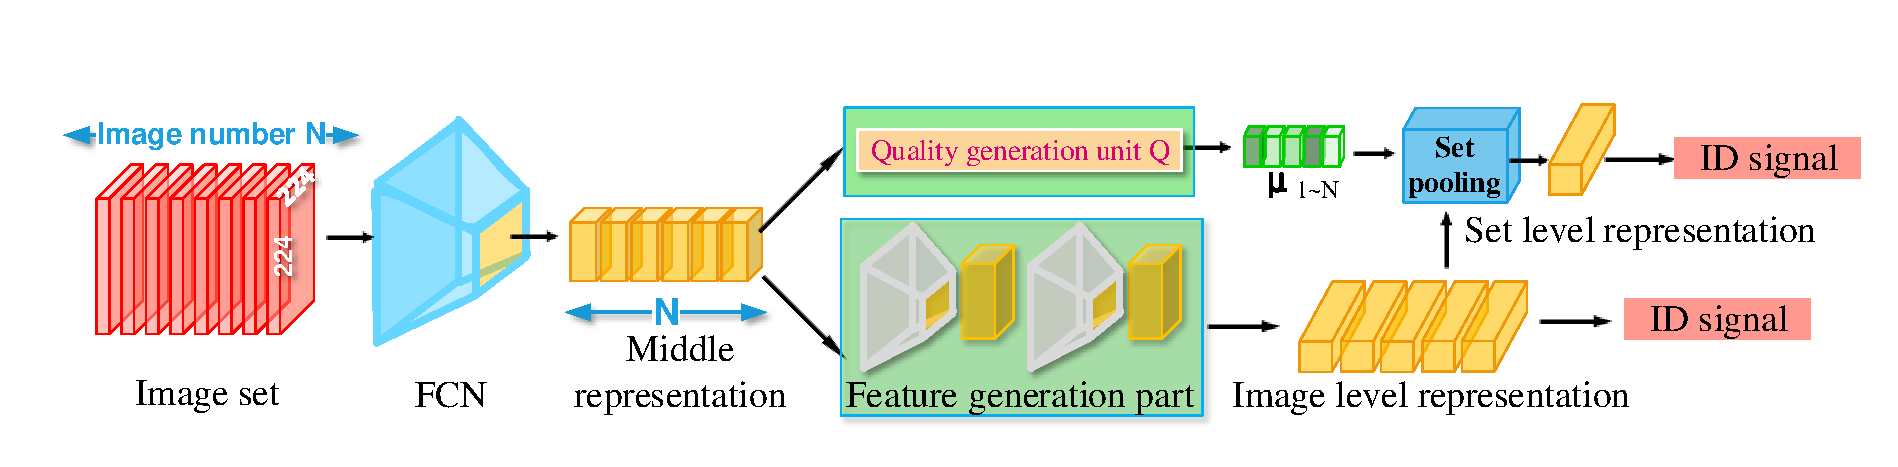
\includegraphics[width=17cm]{figure_train.pdf}
  \caption{The end-to-end learning structure of quality aware net. The input of this structure is three image sets $S_{anchor}$, $S_{pos}$ and $S_{neg}$ belong to class $A$, $A$ and $B$. Each of them pass through the fully convolutional network (FCN) to generate the middle representations, which will be fed to quality generation part and feature generation part. The former generates quality score for each image and the latter generates final representation for each image. Then the scores and representations of all image will be aggregated by set pooling unit and the final representation of the image set will be produced. We use softmax-loss and triplet-loss to be the supervised ID signal. }
\label{figure_train}
\end{figure*}


The proposed QAN belongs to the second approach. It 
discards the dross and selects the essential information in all images. Different from recent works which learn aggregation based on fixed feature \cite{yang2016neural} or image\cite{hassner2016pooling}, the QAN learns feature representation and aggregation simultaneously.  \cite{goswami2014mdlface} proposed a similar quality aware module named ``memorability based frame selection'' which  takes ``visual entropy'' to be the score of a frame. But the score of a frame is defined by human and independent with feature generation unit. In QAN,  score is automatically learned and quality generation unit is joint trained with feature generation unit. Due to mutual benefit between the two parts during training, performance is improved significantly by jointly optimizing images aggregation parameter and images' feature generator.


%Among most of the recent works on set to set recognition, there are two different way to deal with it. One of them directly handles it in a convex hull\cite{cevikalp2010face} or affine hull\cite{hu2011sparse} or subspace\cite{basri2011approximate, Huang2015Projection} expanded by sample' representations in Hilbert space or Grassmann manifold so that this issue can be formulated as a metric learning problem between two hulls, spaces or manifolds\cite{lu2015multi,yang2013face}.  
%
%The others want to predigest the issue to point to point recognition, so they usually try to down-sample or pooling point group to a single point in hyperspace. Bag of features\cite{lazebnik2006beyond}, which is the most famous feature aggregation method, uses histogram to represent the whole set. Another classical work \cite{jegou2010aggregating} proposed vector of locally aggregated descriptors (VLAD), which can aggregate all local discripters from all samples. Temporal max/average pooling are used in\cite{wu2016deep} to integrate all frames' features generated by recurrent convolutional network, which can be seen as using 1st order statistics to pool the set. And 2nd order statistics is used in \cite{wang2012covariance, Zhu2013From} with assuming that the distribution of samples are Gaussians. In \cite{hassner2016pooling}, original faces in a set classified into 20 bins based on their pose and quality. Then faces in each bin are pooled to generate feature and finally feature vectors of all bins are merged to recognition.
%\cite{yang2016neural} uses attention mechanism to summarize several sample points to a single aggregated point. 
%
%These algorithms propel the development of set to set recognition. However, some of them learn the best metric between two sets, but they are always based on strong assumptions and do not make the full use of all samples' information. Some of others learn aggregation methods on fixed feature\cite{yang2016neural} or image\cite{hassner2016pooling} to summarize a set to a point, but they fix the representation of images. The rest of them  neither learn the feature nor learn the aggregation method but just use human designed statistic methods to summarize the set. To learn a better aggregation method and representation synchronously, we propose a quality aware network that can jointly optimizes both aggregation parameter and image's feature generator, and these two parts can benefit from each other during training phase. Finally, image representations are weighting pooled by qualities to be the set representation.
%
%%Face verification and human re-identification are two main methods for biology recognition. Multiple works\cite{sun2014deep,sun2015deeply,taigman2014deepface,facenet,chen2012bayesian
%%,li2014deepreid,zheng2011person,farenzena2010person,gong2014person} have been done on image based recognition. The best accuracy achieved by machine on the most challenge image-based face verification benchmark LFW\cite{learnedlabeled} has been promoted to 99.78\%. In present world, however, set to set recognition is more challenge and useful. 
%%Related works of the paper includes set based recognition, and deep learning based face verification and person re-identification.
%
%%%% ADD more related works for set to set recognition
%
%%Works for set based recogition includes the parametric \cite{arandjelovic2005face,hadid2004still,lee2003video,shakhnarovich2002face} and non-parametric \cite{cevikalp2010face,fan2011margin,harandi2011graph,kim2007discriminative,wang2008manifold} based methods. Parametric methods use image set to estimate a parametric family of distributions and then use the distance defined on probabilistic distributions are used to measure similarity of two sets. The non-parametric methods use geometrical information to measure similarity between two sets. Most of these methods take an image set as a linear subspace and can loss information for discriminative classification. In \cite{yang2016neural}, an attention module is used to aggregated features from image sets.
%
%%Face verification and person re-identification has been well explored, and the accuracy improves significantly in recent years thanks to the deep neural networks and large scale training data. In \cite{taigman2014deepface}, faces are aligned through a 3D shape model and are fed into a network trained by multi-class classification to extract features. Three networks with different alignments and color channels are combined with a SVM with $\chi ^2$ kernel. In \cite{sun2014deep,sun2015deeply}, a more compact and efficient way to extract network features are proposed, where 25 networks are combined with a joint Bayesian based metric learning \cite{chen2012bayesian}. Loss in \cite{sun2014deep,sun2015deeply} are the combined of classification and verification loss. A recent work \cite{schroff2015facenet} use a triplet loss to directly lean a mapping from face images to a compact Euclidean space where distances directly corresponds to a measure of similarity. Deep learning based approaches also achieves leading performance in person re-identification. In \cite{li2014deepreid}, a filter pairing neural network is proposed to jointly handle the misalignment and simultaneously extracts discriminative features. \cite{hu2015deep} proposes the deep transfer metric learning to learn hierarchical transformations for cross domain recognition.  In \cite{ahmed2015improved},  features and a corresponding similarity metric for person re-identification are simultaneously learned.
